%\documentclass[apjl]{emulateapj}
\documentclass[letterpaper,12pt,preprint]{aastex}

% packages
\usepackage{amssymb,amsmath,amsbsy}
\usepackage{booktabs}
\usepackage{multirow}

% commands
\newcommand{\given}{\,|\,}
\newcommand{\dd}{\mathrm{d}}
\newcommand{\transpose}[1]{{#1}^{\mathsf{T}}}
\newcommand{\inverse}[1]{{#1}^{-1}}
\newcommand{\Msun}{\ifmmode {{\rm M}_{\odot}}\else M$_{\odot}$\fi}
\newcommand{\bs}[1]{\boldsymbol{#1}}
\newcommand{\degree}{^{\circ}}
\newcommand{\eqn}{Equation~}

% Symbols
\newcommand{\period}{T_{\rm orb}}
\newcommand{\mf}{M_f}
\newcommand{\wdupper}{1.44}

\begin{document}

\title{The Companion Mass Distribution of extremely low-mass white dwarfs}
\author{Jeff Andrews\altaffilmark{\colum}, Adrian M. Price-Whelan\altaffilmark{\colum}, Marcel Ag\"ueros\altaffilmark{\colum}}

% Affiliations
\newcommand{\colum}{1}
\altaffiltext{\colum}{Department of Astronomy, 
		              Columbia University, 
		              550 W 120th St., 
		              New York, NY 10027, USA}


\begin{abstract}
Measuring the masses of companions to single-line spectroscopic binary stars
is (in general) not possible because of the unknown orbital plane inclination angles. 
Even when the mass of the visible star can be measured, only a lower limit can be placed
on the mass of the unseen companion. However, since the orbital geometry of the systems should be isotropically
distributed, for a large enough, unbiased sample, the 
companion mass distribution can be deconvolved from the distributions of observables.
In this work, we construct a hierarchical probabilistic model to infer properties of unseen 
companion stars given orbital period and projected radial velocity measurements of the primary. We use a mixture of 
two Gaussians to model the true companion mass distribution to represent 
populations of white dwarfs (WD) and neutron stars (NS). We run this model on mock data sets in order to test the
robustness of our inferences. We then apply our model to 55 of the 61 white dwarfs in 
the extremely low mass (ELM) WD survey. We find maximum a posteriori (MAP) parameters for
the WD companion population of $\mu_{\rm WD} = 0.73~\Msun$ and $\sigma_{\rm WD} = 0.26~\Msun$ 
with a NS fraction consistent with zero, $f_{\rm NS} = 0\%$. However, the marginal posterior 
distribution over NS fraction has a significant tail up to $f_{\rm NS} \approx 12\%$.
We make samples from the posterior distribution publicly available and provide a  
script for computing the probability that a ... in the context of our model.
\end{abstract}


\section{Introduction}

The dramatic increase in the number of spectroscopically confirmed white dwarfs (WDs) is seen in the most recently compiled sample from Data Release 7 (DR7) of the Sloan Digital Sky Survey (SDSS), which contains $\sim$20,000 confirmed WDs \citep{kleinman13}. While the distribution of hydrogen atmosphere (DA) WD masses is strongly peaked at $0.6~\Msun$, a small but non-negligible number ($\approx$6\%) are seen as low mass WDs (LMWD) with $M<0.4~\Msun$ both in SDSS and elsewhere \citep[e.g., the Palomar Green Survey;][]{liebert05}.


Except in special cases of extreme metallicity \citep{kilic07}, the Galaxy is not old enough to produce WDs with $M<0.5 \Msun$ through single star evolution. These objects are formed through dynamical interactions with another star, in which the primary overfills its Roche lobe in either an unstable, common envelope \citep{vdSluys06}, or a phase of stable but non-conservative mass transfer \citep{woods12}. After the primary has become a WD, the secondary overfills its Roche lobe, forming a common envelope prior to core helium ignition, leaving a He-core WD secondary in a tight orbit with either a He- or CO- core WD \citep{han98,nelemans00,nelemans01}.


In their seminal work, \citet{marsh95} discovered companions around five LMWDs in their sample of seven objects, confirming these theoretical expectations and cementing LMWDs as fruitful targets for binary searches. The Extremely Low Mass (ELM) WD Survey identifies LMWDs in SDSS for spectroscopic follow-up using combined constraints on photometry and reduced proper motions \citep{ELMI}. After their initial investigation found 11 of 12 LMWDs had close binary companions, further radial velocity follow-up has now brought the sample of ELM WDs to 61 systems, 55 of which have measured radial velocity amplitudes and orbital periods \citep{ELMII, ELMIII, ELMIV, ELMV}.


While the orbital periods and radial velocities indicated the companions were most likely WDs, due to the unmeasured inclination angle, these LMWDs could have NS companions \citep{vLeeuwen07}. However, all radio searches for pulsed emission, as well as searches for blackbody X-ray emission from a NS surface have been unsuccessful \citep{agueros09a,agueros09b,kilic13}. Yet, such systems must exist since LMWDs are observed as companions around millisecond pulsars \citep{vKerkwijk96,callanan98,bassa06,antoniadis12}. Finding even one system would be extremely interesting: the NS binaries with WD companions bright enough to detect spectroscopic radial velocity variations have precisely determined NS masses which provide useful insights into the binary evolution processes that form these systems \citep{benvenuto05,smedley14,jia14}


Selecting the most likely candidates for multiwavelength follow-up is crucial. For each WD in a single-line spectroscopic binary, spectroscopic observations provide the orbital period ($\period$), WD mass ($M_1$), and projected orbital velocity ($K=v \sin i$). Using Kepler's third law, we can write the relation between these quantities and the unknown inclination angle as:
\begin{equation}
	\frac{(M_2 \sin i)^3}{\left(M_1+M_2\right)^2} = \frac{\period}{2\pi G} K^3 = \mf \label{eq:massfunc}
\end{equation}
The righthand side of this equation is the well-known mass function ($\mf$). $M_2$ is minimized for an edge-on orbit, with $i = 90\degree$. Because of the dependence on $i$, the nature of the companion cannot usually be determined based on $\mf$ alone. Figure~\ref{fig:Porb-M1} shows that the population of LMWD with pulsar companions (triangles) occupy the same region in $M_1 - \period$ space as those with WD companions (circles). Therefore, barring rare circumstances (such as an edge-on, eclipsing system), individual LMWDs with NS companions cannot be readily identified.


55 of the 61 systems have precise $M_1$, $\period$, and $K$ measured; we refer to this as the ELM sample. Since the population was selected based on characteristics determined by the primary mass alone, at least with regard to the inclination angle and companion mass, the population is unbiased. In this work, we develop a probabilistic model to infer parameters of an assumed form for the mass distribution of companions to ELM WDs. Our method is similar to that employed by \citet{ozel12} and \citet{kiziltan13} to describe the mass distribution of NSs in binaries. We focus on several specific scientific questions: 1.\ Can the population as a whole be modeled using a simple description of the companion masses? 2.\ How does the companion mass distribution compare to predictions from population synthesis simulations?  3.\ What is the rate of NS-LMWD binaries implied by our model? 4.\ What are the resulting distributions of NS probabilities for individual systems in the ELM sample? 


To answer these questions, we build the mathematical framework in Section 2 that we employ in our model described in Section 3. We give the results and discussion in Section 4, and conclude in Section 5.

\begin{figure}[h!]
\begin{center}
\includegraphics[angle=90,width=0.95\columnwidth]{Porb_M1.eps}
\caption{The $\period$ - $M_1$ distribution of the ELM WD sample. The three eclipsing systems, with known $M_2$ are shown by the filled circles. Arrows indicate the masses of ELM WDs without detected radial velocity variation. Triangles indicate the positions of the known WD-NS binaries. From $\period$ and $M_1$ alone, the two populations are indistinguishable.}
\label{fig:Porb-M1}
\end{center}
\end{figure}




\section{Methods}

We construct a statistical model to derive constraints on a parametric model for the distribution of ELM WD companion masses, $p(M_2 \given \bs{\theta})$.\footnote{In what follows, vectors or sets of parameters or quantites are represented by bold symbols.} For each system, we assume we are given $K$, $T$, and $M_1$ and therefore know the value of the mass function, $\mf$ (\eqn~\ref{eq:massfunc}). We would like to derive posterior constraints on the parameters, $\bs{\theta}$, that describe the distribution of companion masses, $p(M_2\given \bs{\theta})$, given all of the observed mass functions, $\bs{m}_f$, by deconvolving the distribution of mass functions from the unobserved inclination angle, $i$. Using Bayes' rule,
\begin{equation}
    p(\bs{\theta} \given \mf) = \frac{1}{\mathcal{Z}}~p(\mf \given \bs{\theta})~p(\bs{\theta}).
\end{equation}
where $p(\mf \given \bs{\theta})$ is the likelihood, $p(\bs{\theta})$ is the prior on parameters $\bs{\theta}$, and the evidence integral, $\mathcal{Z}$, is a constant that depends only on the data. The marginal likelihood, $p(\mf \given \bs{\theta})$, involves integrals over the latent variables $i$ and $M_2$,
\begin{align}
    p(\mf \given \bs{\theta}) &= \int_0^{\pi/2} di \int_{-\infty}^\infty dM_2  \nonumber \\
      & \qquad {} \times p(\mf \given M_1, M_2, i)~p(M_2 \given \bs{\theta})~p(i).
\end{align}
We neglect observational uncertainties in $\mf$ and $M_1$,\footnote{This is justified because the relative uncertainties in these quantities are small, $\sigma_x / x \sim 0.05-0.1$.} and assume the inclination angles are isotropically distributed
\begin{align}
	p(\mf \given M_1, M_2, i) &= \delta \left[\mf - f(M_1, M_2, i) \right]\\
	f(M_1, M_2, i) &= \frac{(M_2 \sin i)^3}{(M_1 + M_2)^2}\\
	p(i) &= \sin i.
\end{align}
For now, we keep this general by not yet specifying a parametric form for the companion mass distribution, $p(M_2 \given \bs{\theta})$. With the above assumptions, the marginal likelihood integral is
\begin{align}
%    p(\mf \given \bs{\theta}) &= \int_{0}^\infty dM_2~p(M_2 \given \bs{\theta}) \int_0^{\pi/2} di \nonumber \\
%    & \qquad {} \times \delta \left[\mf - f(M_1, M_2, i)\right]~\sin i\\
    p(\mf \given \bs{\theta}) &= \int_{0}^\infty dM_2 ~p(M_2 \given \bs{\theta}) \int_0^{\pi/2} di  \nonumber \\
    & \qquad {} \times ~\sin i ~ \delta \left[g(M_1,M_2,i) \right]\label{eq:delta}
\end{align}
where
\begin{equation}
	g(M_1,M_2,i) = \frac{M_2^3}{(M_1+M_2)^2}\sin^3 i - \mf.
\end{equation}
The inner integral (over $i$) has the form
\begin{equation}
    \int dx~F(x)~\delta \left[ G(x) \right] = \sum_j \frac{F(x^*_j)}{|G'(x^*_j)|}
\end{equation}
where the sum is over the roots, $x^*_j$, of the function $G(x)$. The root, $i^*$, and derivative of the argument of the delta function in \eqn\ref{eq:delta} are 
\begin{align}
%	\sin i^* &= \alpha\\
%	\alpha &= \frac{(\mf(M_1+M_2)^2)^{1/3}}{M_2}\\
	\sin i^* &= \frac{ \left[\mf(M_1+M_2)^2 \right]^{1/3}}{M_2}\\
%	\frac{\partial g}{\partial i} &= \frac{3M_2^3}{(M_1+M_2)^2}\sin^2 i \cos i\\
%	\frac{\partial g}{\partial i}\bigg\rvert_{i^*} &= \frac{3M_2^3}{(M_1+M_2)^2} \alpha^2 \sqrt{1 - \alpha^2}
	\frac{\partial g}{\partial i}\bigg\rvert_{i^*} &= \frac{3M_2^3}{(M_1+M_2)^2} \sin^2 i^* \sqrt{1 - \sin^2 i^*}
\end{align}
With this in mind, we may write the marginal likelihood as
\begin{align}
	p(\mf \given \bs{\theta}) &= \int_{0}^\infty dM_2~p(M_2 \given \bs{\theta})~\sin i^* \left(\frac{\partial g}{\partial i}\bigg\rvert_{i^*}\right)^{-1}\\
%	&= \int_{0}^\infty dM_2~p(M_2 \given \bs{\theta})~\alpha\left[\frac{3M_2^3}{(M_1+M_2)^2} \alpha^2 \sqrt{1 - \alpha^2}\right]^{-1}\\
	&= \int_{M_{2,{\rm min}}}^\infty dM_2~p(M_2 \given \bs{\theta})~h(M_2, \mf, M_1) \label{eq:fullm2}
\end{align}

where the bottom bound in the integral in \eqn\ref{eq:fullm2} is set by the minimum companion mass for which the integrand is real, $M_{2,{\rm min}}$ (determined by setting $i=90\degree$ in \eqn\ref{eq:massfunc} and solving for $M_2$), and

\begin{equation}
h(M_2, \mf, M_1) = \frac{(M_1+M_2)^{4/3}}{3\ \mf^{1/3}M_2\sqrt{M_2^2 - \left[ \mf(M_1+M_2)^2 \right]^{2/3}}}
\end{equation}


\subsection{Our Model} \label{sec:experiments}

We must now choose a functional form for the companion mass distribution,  $p(M_2\given \bs{\theta})$. For all experiments -- including that with the real data -- we use a two component Gaussian mixture model to fit the data. However, in tests below, we generate test data with a variety of mixture component forms. We truncate the distributions using physically motivated bounds so that the white dwarf component is restricted to the range $M_2\in (0.2,\wdupper)~\Msun$ and the neutron star component is restricted to the range $M_2\in (1.3,2)~\Msun$,
\begin{align}
%	h(M_2, \mf, M_1) &= \frac{(M_1+M_2)^{4/3}}{3\mf^{1/3}M_2\sqrt{M_2^2 - \left[ \mf(M_1+M_2)^2 \right]^{2/3}}}\\
%	p(\mf \given \bs{\theta}) &= \int_{0}^\infty dM_2~\left[ (1-f_{\rm NS})p_{\rm WD} + f_{\rm NS}p_{\rm NS} \right]~h(M_2, \mf, M_1)\\
	p(M_2 \given \bs{\theta}) &= \left[ (1-f_{\rm NS})p_{\rm WD} + f_{\rm NS}p_{\rm NS} \right] 
\end{align}
where 
\begin{align}
	p_{\rm WD} &= \mathcal{N}(M_2 \given \mu_{\rm WD}, \sigma^2_{\rm WD});\,\left[ 0.2 < \frac{M_2}{\Msun} < \wdupper \right] \\
	p_{\rm NS} &= \mathcal{N}(M_2 \given \mu_{\rm NS}, \sigma^2_{\rm NS});\, \left[1.3 < \frac{M_2}{\Msun} < 2 \right].
\end{align}
and $\mathcal{N}$ is the (truncated, but properly normalized) normal distribution with mean $\mu$ and variance $\sigma^2$ and the distributions are limited to the ranges specified. In this work, we fix the mean and variance of the neutron star distribution to
\begin{align}
	\mu_{\rm NS} &= 1.4~\Msun\\
	\sigma^2_{\rm NS} &= (0.05~\Msun)^2
\end{align}
based on indications that NSs in certain binaries may be somewhat more massive than the canonical NS mass of 1.35 \Msun \citep{kiziltan13,smedley14}. 

%The probability of any particular system having a NS companion $P_{\rm NS}$ is then:

%\begin{equation}
%P_{\rm NS} = \int_{0}^\infty dM_2~ f_{\rm NS}~ \mathcal{N}(M_2 \given \mu_{\rm NS}, \sigma^2_{\rm NS})~ h(M_2, \mf, M_1) \label{eq:P_NS_full}
%\end{equation}

Our companion mass model parameters are then $\bs{\theta} = (\mu_{\rm WD}, \sigma_{\rm WD}, f_{\rm NS})$. We choose standard priors on these parameters: for the mean of the white dwarf component, we use a uniform distribution from $0.2-1.4~\Msun$; we use a (scale-invariant) logarithmic prior for the variance of the white dwarf component over the range $0.05-2~\Msun$; finally, we use a uniform prior over the dimensionless neutron star fraction from $0-1$. The model parameters are summarized in Table~\ref{tbl:parameters}.

\begin{deluxetable}{ccccc}
	\tablecaption{Model Parameters \label{tbl:parameters}}

	\tablehead{
		\multicolumn{2}{c}{} &
		\colhead{$\mu_{\rm WD}$} & 
		\colhead{$\sigma_{\rm WD}$} &
		\colhead{$f_{\rm NS}$} \\
		\colhead{} &
		\colhead{} &
		\colhead{[\Msun]} &
		\colhead{[\Msun]} &
		\colhead{}
	}

	\startdata
		\multicolumn{2}{c}{Priors} & $\mathcal{U}(0.2, 1.4)$ & $\left[\ln(40)\sigma\right]^{-1}$ $(0.05 < \sigma/\Msun < 2)$ & $\mathcal{U}(0, 1)$ \\
		\cutinhead{Test Cases}
		\multirow{2}{*}{Test 1} & True & 0.7 & 0.2 & 0.0 \\
		 & MAP & {\bf XXX} & {\bf XXX} & {\bf XXX} \\
		 \hline
		\multirow{2}{*}{Test 2} & True & 0.7 & 0.2 & 0.1 \\
		 & MAP & {\bf XXX} & {\bf XXX} & {\bf XXX} \\
		 \hline
		\multirow{2}{*}{Test 3} & True & \nodata & \nodata & 0.1 \\
		 & MAP & {\bf XXX} & {\bf XXX} & {\bf XXX} \\
		 \cutinhead{ELM Sample}
		 & MAP & 0.73 & 0.26 & {\bf 5\%?}
	\enddata

	\tablecomments{Parameter information for the form of the companion mass distribution used in the experiments of Section~\ref{sec:experiments}. $\mathcal{U}$ is the uniform distribution. There are 3 free parameters. We additionally fix the NS distribution: $\mu_{\rm NS} = 1.4~\Msun$ and $\sigma_{\rm NS} = 0.1~\Msun.$}\

\end{deluxetable}


We use an ensemble Markov Chain Monte Carlo algorithm \citep{goodman10} to draw samples from the posterior distribution, $p(\mu_{\rm WD}, \sigma_{\rm WD}, f_{\rm NS} \given \bs{m}_f, \bs{M}_1)$. The algorithm is implemented in the \texttt{Python} programming language \citep{foremanmackey13} and uses an ensemble of individual ``walkers'' to naturally adapt to the geometry of the parameter-space being explored. We run the walkers for an initial, burn-in period of 1000 steps starting from randomly drawn initial conditions (sampled from the priors in Table~\ref{tbl:parameters}). We then re-initialized the walkers from their positions at the end of this run, throw out the burn-in samples, and run again for 1000 steps. We compute the autocorrelation time for each parameter to confirm they have converged.


\section{Test Cases} \label{sec:tests}
To test the performance of this Gaussian mixture model, we apply it to three separate sets of mock data (described in detail below), each with 100 ``observed'' systems. These data are generated by randomly drawing the companion mass, $M_2$, from a particular distribution, then using a randomly drawn inclination angle and primary mass, $M_1$, to compute the mass function, $\mf$. We draw primary masses from a uniform distribution, $M_1 \sim \mathcal{U}(0.2,0.4)~\Msun$. We apply the same Gaussian mixture model to all test datasets to infer the parameters of the white dwarf mixture component and neutron star fraction.


\begin{figure*}[h!]
\begin{center}
\includegraphics[width=0.95\textwidth]{many-panel.pdf}
\caption{The model results of our three tests described in Section~\ref{sec:tests}. The left-most panel shows a histogram of the $M_2$ drawn from each of our test distributions. Overplotted as a solid line is posterior distribution using the maximum a posteriori parameter values, resulting from our model. The second panel shows the posterior distributions for $\mu_{\rm WD}$ and $\sigma_{\rm WD}$. The dashed lines in the top two panels show the true values that the sample systems were drawn from. Since the third model was not drawn from a Gaussian distribution, there is no true parameter set. The third panel shows the convolved posterior histogram for $f_{\rm NS}$, with the dashed lines in the bottom two panels showing the true value of 10\%. Finally, the rightmost panels show the NS probability for individual systems as a function of $\mf$. The error bars in $P_{\rm NS}$ enclose the interquartile range.}
\label{fig:tests}
\end{center}
\end{figure*}


\subsection{Test 1: Single Gaussian (white dwarf)} \label{sec:exp1}

As a first test, we generate $M_2$'s by drawing from a single, truncated Gaussian with mean, variance, and bounds
\begin{align}
	\mu_{\rm WD, true} &= 0.7~\Msun\\
	\sigma^2_{\rm WD, true} &= (0.2~\Msun)^2\\
	0.2 < &\frac{M_2}{\Msun} < \wdupper.
\end{align}
This is equivalent to setting the neutron star fraction to $f_{\rm NS} = 0$. 

\subsection{Test 2: Two Gaussians (white dwarf + neutron star)} \label{sec:exp2}
For our next test, we use the same Gaussian distribution to generate companion masses for the white dwarf component as the previous example (Section~\ref{sec:exp1}), but we now add an additional neutron star component with parameters
\begin{align}
	\mu_{\rm NS, true} &= 1.4~\Msun\\
	\sigma^2_{\rm NS, true} &= (0.05~\Msun)^2\\
	1.3 < & \frac{M_2}{\Msun} < 2.
\end{align}
We set the neutron star fraction to $f_{\rm NS} = 0.1$. 

% [TODO: We have also tried changing the mean and variance of the true neutron star distribution while keeping the fitting parameters fixed and found ...]

\subsection{Test 3: Uniform (white dwarf) + Gaussian (neutron star)} \label{sec:exp3}
For a final test, we use the same neutron star component as in Section~\ref{sec:exp2}, but now generate companion masses for the white dwarf component by sampling from a uniform distribution over the range $(0.2,1.2)~\Msun$. We keep the neutron star fraction fixed to $f_{\rm NS}=0.1$. 

\subsection{Test results}
The test results are summarized by Figure~\ref{fig:tests}. Each row corresponds to one of the three tests described above. The left-most column shows the true distribution of $M_2$'s, over-plotted with the maximum a posteriori (MAP) model from our posterior samples, inferred from mock observations of the mass functions, $\mf$, and primary masses, $M_1$, of the mock data. The middle panels show samples from the posterior in two projections (grey points), along with contours that contain 68\% and 95\% of the samples. The final column shows the probability that any given test object is a neutron star, as computed for 512 samples from the posterior.

\section{The ELM Sample}

The ELM WD sample is composed of 55 of 61 systems with radial velocity variations fit to orbital solutions, which provide precise measurements of $\period$ and $K$. Fitting the sample's high S/N spectra to templates provides precisely determine $M_1$ values. We use the spectroscopic solutions found in \citet{gianninas14}. Three systems are eclipsing binaries, with known companion masses (J0345$+$1748: $M_2=0.72~\Msun$ \citep{kaplan14}, J0651$+$2844: $M_2=0.50~\Msun$ \citep{brown11b}, and J0751$-$0141: $M_2=0.97~\Msun$ \citep{kilic14}). For these systems, the likelihood reduces to:
\begin{equation}
p(\mf \given \theta) = (1-f_{\rm NS}) \mathcal{N}(M_2^* \given \mu_{\rm WD}, \sigma^2_{\rm WD})
\end{equation}
where $M_2^*$ is the mass of the WD companion in these three systems. 

The other six systems in the ELM WD sample show no evidence of orbital motion, with radial velocity upper limits of $\approx$20-50 km s$^{-1}$. Some of these systems may be in low inclination angle binaries with radial velocities below the detection limit or have orbital periods near 24 hours, which are difficult to detect \citep{ELMV}. These LMWDs could also have companions at systematically longer orbital periods, with orbital velocities below the detection limit. Because of the uncertainties in their formation, we remove these from our analysis.




\begin{figure*}[h!]
\begin{center}
\includegraphics[width=0.95\textwidth]{real-data.pdf}
\caption{The posteriors for our model applied to the ELM WDs. The first panel shows the distribution of $M_2$ for the data set. The black line gives the maximum a posteriori value, while the fainter lines show a set of randomly selected realizations from our model. The second panel shows the posterior distribution of $\mu$ and $\sigma$; The maximum a posteriori Gaussian model has $\mu_{\rm WD}= 0.74~\Msun$ and $\sigma_{\rm WD}= 0.26~\Msun$. The third panel shows a NS fraction consistent with zero, however with a non-negligible tail toward higher NS probabilities. This is further indicated by the fourth panel in Figure \ref{fig:ELM_post} which shows the relation between $\mf$ and $P_{\rm NS}$ for individual systems. }
\label{fig:ELM_post}
\end{center}
\end{figure*}



\section{Results and Discussion}

The results of our model are shown in Figure \ref{fig:ELM_post}. The maximum a posteriori Gaussian model has $mu_{\rm WD} = {\bf 0.74} \Msun$ and $\sigma_{\rm WD} = {\bf 0.26}~\Msun$. While the well-defined peak in the posterior distribution demonstrates convergence of the model, the extended distribution toward larger variances could indicate that the true distribution does not match a Gaussian. However it is interesting that the best fit Gaussian for the companions to the ELM WD sample is similar to that of the population of single DA WDs in SDSS with a mean of 0.6 $\Msun$ \citep{kleinman13}. Our distribution is significantly wider ({\bf $\sigma \approx 0.26~\Msun$} compared with $\sigma \approx 0.1~\Msun$), likely due to mass transfer affecting the mass distribution of the unseen primary WDs as well.


Our results are independent of astrophysical expectations since they do not include any priors on $\mu_{\rm WD}$ and $\sigma_{\rm WD}$, apart from limits for $M_2$ of 0.2 \Msun (based on observations of LMWDs) and \wdupper \Msun (based on the Chandrasekhar mass). In principle, priors could be added based on population synthesis models which suggest there are two dominant companion populations to LMWDs, composed of CO and He core WDs \citep{han98}. The ratio and distribution of these two populations depends on the exact stellar evolution prescriptions assumed \citep[see discussion in, e.g., ][]{toonen12}. Our model could be expanded to include a two Gaussian model --- one for each WD population. The ratio of these populations could potentially place an important constraint on population synthesis models. However, we have found that there is not enough data to motivate adding additional freedom to the model in the form of a second WD component.


The third panel in Figure~\ref{fig:ELM_post} shows a NS fraction strongly peaked toward zero, however there is a significant tail toward higher NS probabilities. Our model does indicate an upper limit to the NS fraction of {\bf XXX\%} at the 95\% confidence level. For 55 systems with observed radial velocity variations, this corresponds to a {\bf 0-4?} systems with NS companions. These results are in agreement with independent constraints from \citet{vLeeuwen07} who set an upper limit on $f_{\rm NS}$ of 18$\pm5$\% based on the non-detection of radio emission from eight LMWD targets. With non-detections of radio emission from an expanded sample of 15 LMWD targets in the ELM WD sample, \citet{agueros09b} place a more stringent upper limit on $f_{\rm NS}$ of $10\substack{+4 \\ -2}\%$. 


Since our results are still consistent with a 0\% NS fraction, it is not guaranteed that any of the LMWDs in the ELM WD sample have NS companions. However the fourth panel in Figure \ref{fig:ELM_post} indicates which ELM WDs have the highest probability of hosting NS companions. Here, we show the relation between $\mf$ and $P_{\rm NS}$ for individual systems. This panel shows that $P_{\rm NS}$ only starts to significantly deviate from zero for {\bf $\mf\approx0.6 \Msun$} Although a few systems have high probabilities, the distribution is strongly clustered near 0\%.


The two systems with $P_{\rm NS}$ above {\bf 10\%} are J0811$+$0225 ({\bf XXX}\%) and J1741$+$6526 ({\bf XXX}\%). These systems are ideal candidates for searches for NS companions in radio and X-ray. Radio observations of these objects are in progress, however because a NS companion may be radio quiet or beamed away from us, a NS companion to these LMWDs may not be detectable in radio \citep{vLeeuwen07}. All NS give off blackbody radiation peaked in X-ray wavelengths, therefore X-ray follow-up provides a more stringent test on the potential for a NS companion \citep{agueros09a}. Previous searches for LMWDs with X-ray counterparts have all been non-detections, however we show here that all those sources have a low probability of hosting a NS companion. If J0811$+$0225 and J1741$+$6526 also lack X-ray counterparts, then even more stringent constraints can be placed on $f_{\rm NS}$. In future work, we plan to combine these results with radio and x-ray non-detections to further constrain $P_{\rm NS}$ for each system. 


It is worth noting that the fourth panels in our test cases in Figure~\ref{fig:tests} shows that our model is fairly good at identifying those systems most likely to host NS's. However it also shows that roughly half of the LMWDs with NS companions may appear with a deceptively low $f_{\rm NS}$ due to the inclination angle. Systems with NS companions cannot all be differentiated from those with WD companions through the mass function and LMWD mass alone. Therefore there is a non-negligible probability that {\it any} LMWD could host a NS companion.


The probability of any particular ELM WD having a NS companion will vary depending on the NS fraction of the sample. This is not taken into account in \eqn\ref{eq:P_NS_approx}. {\bf TEXT ON USING PYTHON SCRIPT FOR DETERMINING P-NS FOR FUTURE DISCOVERED LMWDs.}


Recently, \citet{hermes14} made high-speed photometric observations of 20 LMWDs in the ELM sample to search for eclipses. They placed limits on the maximum inclination angle of these 20 systems based on the non-detection of eclipses. For eight objects they determined the companion mass based on models fitting the observed photometric variability, primarily due on ellipsoidal variation and doppler beaming. We have not included these observations in our model, but we plan to explore this in future work.





%%%%%%%%%%%%%%%%%%%%%%%%%%%%
%
% If we do this calculation, we need to think more about it
% 
%%%%%%%%%%%%%%%%%%%%%%%%%%%%

%Combining our resulting NS fraction of {\bf 5\%} with the ELM WD space density of 40 kpc$^{-3}$ as determined by \citet{brown11a}, we can find a space density of ELM WD + NS binaries of 2 kpc$^{-3}$. If we assume an exponential disk with a scale height of 250 pc, this suggests that there are $\approx$  such binaries within a two kpc of us. Compare to the number of known MSP+LMWDs.


%%%%%%%%%%%%%%%%%%%%%%%%%%%%%%%%%%
%
%  If we say anything about non-detections, we need to fix up the
% math below. I suggest we wait and discuss these in a future work
%
%%%%%%%%%%%%%%%%%%%%%%%%%%%%%%%%%%

%\subsection{Non-detections}

%Six systems in the ELM WD sample have non-detections of companions, down to an upper limit on the transverse velocity. We include these systems in our model, too, as in principle they could be binary systems at with low inclination angles or long period orbits or both. We can estimate the number of binaries with inclination angles too low to produce observable radial velocity variations:

%\begin{equation}
%P(K<K_{\rm max} | \mathbf{\Theta}) = \int_0^{\infty} \int_0^{i_{\rm max}} P(M_2|\mathbf{\Theta})\ {\rm sin}\ i\ {\rm d}i\ {\rm d}M_2
%\end{equation}

%which reduces to:

%\begin{equation}
%P(K<K_{\rm max} | \mathbf{\Theta}) = \int_0^{\infty} P(M_2|\mathbf{\Theta})\ \left( 1 - {\rm cos}\ i_{\rm max}\right)\ {\rm d}M_2
%\end{equation}

%where $i_{\rm max}$ is the smallest inclination angle that would still produce an unobservable binary, found by solving equation 1, using $K_{\rm max}$ for $K$. For an estimate of the expected fraction of unobserable binaries, we adopt $0.25~\Msun$ for $M_1$, an orbital period of 0.5 days, and a limiting velocity of 50 km s$^{-1}$. For our best fit model, with $\mu=0.6$, $\sigma=0.3$, and $\mathcal{f}=0.03$, we numerically calculate the integral above, and find that we would expect $\sim$2\% and $\sim$7\% of systems to have radial velocity variations below 25 km s$^{-1}$ and 50 km s$^{-1}$, respectively. If we increase the fiducial orbital period to 1.0 day, those numbers increases to 3\% and 10\%, respectively. For the ELM sample with 61 systems, this corresponds to 2 and 6 systems, consistent with the number of non-detections observed. Although we caution that this result is based on our imperfect model, it suggests that the number of non-detections observed is consistent with binaries at low inclination angles (albeit at slightly larger orbital periods than that of the observed population).


\section{Conclusions}

\begin{enumerate}
\item We have created a mathematical description to describe the companion mass distribution of a set of unbiased single-lined spectroscopic binaries. \\
\item We have used that mathematical framework to build a Markov Chain Monte Carlo model and applied it to the set of WDs from the ELM WD survey. \\
\item Our model suggests that the majority of ELM WDs have CO-core WDs. This is in contrast to predictions from population synthesis models. In a future work, we plan to quantify the ratio of He+He core WDs to He+CO core WDs. \\
\item Our model indicates that the fraction of ELM WDs with NS companions is of order a few percent. We provide an updated formula for determining the probability of any particular LMWD having a NS companion. We further identify J0811$+$0225 and J1741$+$6526 as having the highest probabilities of hosting a NS companion with {\bf XXX\%} and {\bf XXX\%}, respectively. \\
\end{enumerate}

\acknowledgements
The authors wish to acknowledge David Hogg (NYU) for useful discussions, and the organizers of the \emph{AstroData Hack Week} (2014). 
APW is supported by a National Science Foundation Graduate Research Fellowship under Grant No.\ 11-44155. 
This research made use of Astropy, a community-developed core \texttt{Python} package for Astronomy \citep{astropy13}. \\

\bibliographystyle{apj}
\bibliography{refs}
  
\bibitem[Goodman~\&\ Weare(2010)]{goodman10}
Goodman,~J. \& Weare,\ J.,
2010, Comm.\ App.\ Math.\ Comp.\ Sci., 5, 65




\end{document}

